% This file was created by matplotlib2tikz v0.6.18.
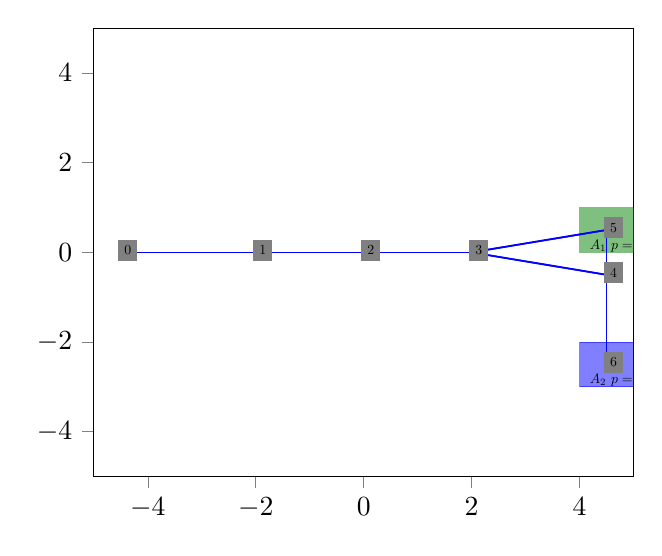
\begin{tikzpicture}

\begin{axis}[
tick align=outside,
tick pos=left,
x grid style={lightgray!92.02614379084967!black},
xmin=-5, xmax=5,
y grid style={lightgray!92.02614379084967!black},
ymin=-5, ymax=5
]
\addplot [only marks, draw=green!50.0!black, fill=green!50.0!black, colormap/viridis]
table [row sep=\\]{%
x                      y\\ 
};
\path [draw=green!50.19607843137255!black, fill=green!50.19607843137255!black, opacity=0.5] (axis cs:5,-4.93038065763132e-31)
--(axis cs:5,1)
--(axis cs:4,1)
--(axis cs:4,-3.94430452610506e-31)
--cycle;

\path [draw=blue, fill=blue, opacity=0.5] (axis cs:5,-3)
--(axis cs:5,-2)
--(axis cs:4,-2)
--(axis cs:4,-3)
--cycle;

\addplot [semithick, blue, forget plot]
table [row sep=\\]{%
-4.5	0 \\
-2	0 \\
};
\addplot [semithick, blue, forget plot]
table [row sep=\\]{%
-2	0 \\
-4.5	0 \\
};
\addplot [semithick, blue, forget plot]
table [row sep=\\]{%
-2	0 \\
0	0 \\
};
\addplot [semithick, blue, forget plot]
table [row sep=\\]{%
0	0 \\
-2	0 \\
};
\addplot [semithick, blue, forget plot]
table [row sep=\\]{%
0	0 \\
2	0 \\
};
\addplot [semithick, blue, forget plot]
table [row sep=\\]{%
2	0 \\
0	0 \\
};
\addplot [semithick, blue, forget plot]
table [row sep=\\]{%
2	0 \\
4.5	-0.5 \\
};
\addplot [semithick, blue, forget plot]
table [row sep=\\]{%
2	0 \\
4.5	0.5 \\
};
\addplot [semithick, blue, forget plot]
table [row sep=\\]{%
4.5	-0.5 \\
2	0 \\
};
\addplot [semithick, blue, forget plot]
table [row sep=\\]{%
4.5	-0.5 \\
4.5	0.5 \\
};
\addplot [semithick, blue, forget plot]
table [row sep=\\]{%
4.5	-0.5 \\
4.5	-2.5 \\
};
\addplot [semithick, blue, forget plot]
table [row sep=\\]{%
4.5	0.5 \\
2	0 \\
};
\addplot [semithick, blue, forget plot]
table [row sep=\\]{%
4.5	0.5 \\
4.5	-0.5 \\
};
\addplot [semithick, blue, forget plot]
table [row sep=\\]{%
4.5	-2.5 \\
4.5	-0.5 \\
};
\node at (axis cs:-4.54,-0.05)[
  scale=0.5,
  fill=lightgray!66.92810457516339!black,
  draw=lightgray!66.92810457516339!black,
  line width=0.4pt,
  inner sep=4pt,
  anchor=base west,
  text=black,
  rotate=0.0
]{ 0};
\node at (axis cs:-2.04,-0.05)[
  scale=0.5,
  fill=lightgray!66.92810457516339!black,
  draw=lightgray!66.92810457516339!black,
  line width=0.4pt,
  inner sep=4pt,
  anchor=base west,
  text=black,
  rotate=0.0
]{ 1};
\node at (axis cs:-0.04,-0.05)[
  scale=0.5,
  fill=lightgray!66.92810457516339!black,
  draw=lightgray!66.92810457516339!black,
  line width=0.4pt,
  inner sep=4pt,
  anchor=base west,
  text=black,
  rotate=0.0
]{ 2};
\node at (axis cs:1.96,-0.05)[
  scale=0.5,
  fill=lightgray!66.92810457516339!black,
  draw=lightgray!66.92810457516339!black,
  line width=0.4pt,
  inner sep=4pt,
  anchor=base west,
  text=black,
  rotate=0.0
]{ 3};
\node at (axis cs:4.46,-0.55)[
  scale=0.5,
  fill=lightgray!66.92810457516339!black,
  draw=lightgray!66.92810457516339!black,
  line width=0.4pt,
  inner sep=4pt,
  anchor=base west,
  text=black,
  rotate=0.0
]{ 4};
\node at (axis cs:4.46,0.45)[
  scale=0.5,
  fill=lightgray!66.92810457516339!black,
  draw=lightgray!66.92810457516339!black,
  line width=0.4pt,
  inner sep=4pt,
  anchor=base west,
  text=black,
  rotate=0.0
]{ 5};
\node at (axis cs:4.46,-2.55)[
  scale=0.5,
  fill=lightgray!66.92810457516339!black,
  draw=lightgray!66.92810457516339!black,
  line width=0.4pt,
  inner sep=4pt,
  anchor=base west,
  text=black,
  rotate=0.0
]{ 6};
\node at (axis cs:4.1,0.07)[
  scale=0.5,
  anchor=base west,
  text=black,
  rotate=0.0,
  align=left
]{ $A_1$
$p=0.3$};
\node at (axis cs:4.1,-2.93)[
  scale=0.5,
  anchor=base west,
  text=black,
  rotate=0.0,
  align=left
]{ $A_2$
$p=0.6$};
\end{axis}

\end{tikzpicture}